\section{Aplicaciones de las redes neuronales}
\subsection{Feedforward}
\begin{itemize}
    \item Estas redes son útiles para tareas en las que hay que aprender una relación entre entradas y salidas, típicamente:
    \item Clasificación de imágenes: Reconocimiento de productos, detección de defectos en imágenes.
    \item Predicción de series temporales: Pronósticos de ventas, análisis del mercado bursátil, gestión energética.
    \item Detección de fraudes: Identificación de transacciones fraudulentas en tarjetas de crédito.
\end{itemize}
\subsection{Redes Neuronales Recurrentes (RNN)}
Permiten procesar secuencias de datos, ya que la información se retroalimenta a través de bucles en la red.

Se usan comúnmente para problemas ordinarios o temporales como, por ejemplo, la traducción de idiomas, el procesamiento del lenguaje natural (NLP), el reconocimiento de voz y los subtítulos de imágenes; se incorporan a aplicaciones populares como Siri y Google Translate.

Algunas aplicaciones típicas:
Traducción automática: Traducción de textos de un idioma a otro.

Reconocimiento de voz: Conversión de voz a texto.

Análisis de sentimientos: Detección de emociones en textos o publicaciones en redes sociales.
\subsection{Hopfield}
La Red de Hopfield es una red recurrente, es decir, existe realimentación entre las neuronas. De esta forma, al introducir un patrón de entrada, la información se propaga hacia adelante y hacia atrás, produciéndose una dinámica. En algún momento, la evolución se detendrá en algún estado estable. En otros casos, es posible que la red no se detenga nunca.

Las aplicaciones típicas de las Redes Hopfield incluyen el reconocimiento de patrones, la memoria direccionable por contenido y la optimización .

\section{Red neuronal convolucional para la detección y clasificación del cáncer de mama mediante aprendizaje profundo}
El estudio presenta una nueva arquitectura de CNN llamada BCCNN, diseñada para detectar y clasificar imágenes de cáncer de mama en ocho clases distintas (presumiblemente diferentes tipos o estados de tumores). El objetivo es mejorar la precisión y versatilidad en el diagnóstico, y demostrar que una CNN con mecanismos de regulación de aprendizaje puede alcanzar resultados clínicamente útiles.
\subsection{Datos y procesamiento}

Orígenes del dataset: Obtienen imágenes de mamografías a partir de bases públicas en Kaggle (como CBIS-DDSM, MiniDDSM y otras) .
Estas bases incluyen imágenes originales junto con etiquetas clínicas (benigno, maligno, subcategorías).

Preprocesamiento:
Normalización del tamaño y contraste.
Aumento de datos: rotaciones, espejos y escalados para ampliar el set y evitar sobreajuste.

\textbf{Clases de tumeres identificadas:}
\begin{itemize}
    \item BA (adenosis benigno)
    \item BF (fibroadenoma benigno)
    \item BPT (tumor benigno de phyllodes)
    \item BTA (adenoma tubular benigno)
    \item MDC (carcinoma ductal maligno)
    \item MLC (carcinoma lobular maligno)
    \item MMC (carcinoma mucinoso maligno)
    \item MPC (carcinoma papilar maligno)
\end{itemize}
\begin{figure}
    \centering
    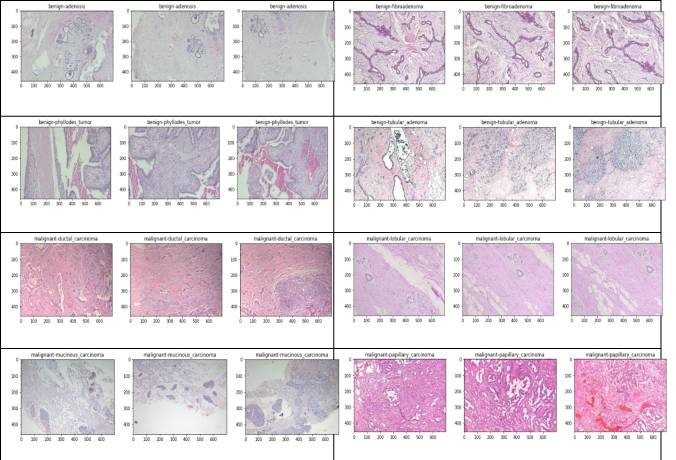
\includegraphics[width=0.5\linewidth]{cancer.jpg}
    \caption{}
    \label{fig:enter-label}
\end{figure}


\subsection{Arquitectura}
\begin{itemize}
    \item Entrada

Imagen de RM (resonancia) con distintas magnificaciones (40x–400x).

\item Capas Convolucionales 
Varias capas CNN que extraen características visuales progresivas (texturas, formas).

No se especifican filtros exactos, pero siguen un patrón típico de extracción jerárquica.

\item Pooling

Capas de max pooling para reducir la información espacial y concentrar lo relevante.

\item Flatten

Convierte los mapas de características en un vector 1D.

\item Capas Fully Connected

Una o más capas densas que combinan las características para clasificación.

\item Capa de salida (Softmax)

8 neuronas (una por clase), con función softmax para obtener la probabilidad de cada tumor.


    
\end{itemize}
\subsection{Comparación con otros modelos}
El artículo también evalúa y compara BCCNN con seis modelos pre-entrenados en ImageNet:

Xception,InceptionV3,VGG16,MobileNet,ResNet50.

Realizan un total de 30 experimentos, combinando los seis modelos con las cinco magnificaciones de imagenes (40x–400x)
\subsection{Resultados}
F1-score del BCCNN: $98.28\%.$

Comparado con los demás:

ResNet50: $98.14\%$

VGG16: $97.67\%$

Xception: $97.54\%$

MobileNet: $93.98\%$

Esto muestra que su arquitectura personalizada logró resultados ligeramente mejores que modelos grandes preentrenados .

